\documentclass[
	% -- opções da classe memoir --
	11pt,				% tamanho da fonte
	openright,			% capítulos começam em pág ímpar (insere página vazia caso preciso)
	oneside,			% para impressão em recto e verso. Oposto a oneside
	a4paper,			% tamanho do papel. 
	%fleqn,              % Neto - Tentando alinhar todas as equacoes
	% -- opções da classe abntex2 --
	chapter=TITLE,		% títulos de capítulos convertidos em letras maiúsculas
	section=TITLE,		% títulos de seções convertidos em letras maiúsculas
	%subsection=TITLE,	% títulos de subseções convertidos em letras maiúsculas
	%subsubsection=TITLE,% títulos de subsubseções convertidos em letras maiúsculas
	sumario=abnt-6027-2012,
	% -- opções do pacote babel --
	english,			% idioma adicional para hifenização
	french,				% idioma adicional para hifenização
	spanish,			% idioma adicional para hifenização
	brazil				% o último idioma é o principal do documento
	]{abntex2}

% ---
% Pacotes básicos 
% ---
% \usepackage{times}
\usepackage{tgschola}
% \usepackage{utopia}
\usepackage[T1]{fontenc}		% Selecao de codigos de fonte.
\usepackage[utf8]{inputenc}		% Codificacao do documento (conversão automática dos acentos)
\usepackage{indentfirst}		% Indenta o primeiro parágrafo de cada seção.
\usepackage{color}				% Controle das cores
\usepackage{graphicx}			% Inclusão de gráficos
\usepackage{microtype} 			% para melhorias de justificação
% ---
		
% ---
% Pacotes adicionais
% ---
\usepackage{mathtools}
\usepackage{booktabs}
\usepackage{amsmath,amsthm,amsfonts,cite,color,enumerate,subfig}
\usepackage{mathrsfs}
\usepackage{enumitem}
\usepackage{nicefrac}
\usepackage{subfig}
\usepackage{algpseudocode}
\usepackage{pdflscape}
\usepackage{pdfpages}
\usepackage{framed}
\usepackage{cancel} % Use \usepackage[thicklines]{cancel} for thicker strokes

\usepackage{lipsum}  % for sample text

\usepackage[font=small, position=top]{caption}

\newenvironment{openingquote}
    {
        \begin{flushright}
        \begin{minipage}{\textwidth - 4cm}
        \small
    }
    { 
        \end{minipage}
        \end{flushright}
    }

\definecolor{cancelgray}{gray}{0.5}
\renewcommand{\CancelColor}{\color{cancelgray}}

\usepackage{geometry}
\geometry{
    a4paper,
    left=30mm,
    top=30mm,
    right=20mm,
    bottom=20mm,
}
\linespread{1.5}
\usepackage{chngcntr}
\counterwithout{equation}{chapter} % remove the chapter number

\newtheorem{theorem}{Theorem}
\newtheorem{example}{Example}
\newtheorem{corollary}{Corollary}
\newtheorem{definition}{Definition}
\newtheorem{algorithm}{Algorithm}
\newtheorem{lem}[theorem]{Lemma}
\allowdisplaybreaks

% NEW COMMANDS
\renewcommand{\mod}[1]{\  (\mathrm{mod} \ #1)}
\newcommand{\qi}{\boldsymbol{i}}
\newcommand{\qphi}{\boldsymbol{\phi}}
\newcommand{\qj}{\boldsymbol{j}}
\newcommand{\qk}{\boldsymbol{k}}
\newcommand{\qmu}{\boldsymbol{\mu}}
\newcommand{\qnu}{\boldsymbol{\nu}}
\newcommand{\qV}{\boldsymbol{V}}
\newcommand{\sen}{\mathrm{\, sen \,}}
\newcommand{\red}[1]{{\color{red}#1}}
\DeclareRobustCommand{\rchi}{{\mathpalette\irchi\relax}}
\newcommand{\irchi}[2]{\raisebox{\depth}{\Large $#1\chi$}} % inner command, used by \rchi
\newcommand{\floatsource}[1][the author (2022)]{\\ \small Source: #1.}

% ISOMORPHISM SYMBOL
\makeatletter
\newcommand*{\isomorphism}{%
	\mathrel{%
		\mathpalette\@isomorphism{}%
	}%
}
\newcommand*{\@isomorphism}[2]{%
	% Calculate the amount of moving \sim up as in \simeq
	\sbox0{$#1\simeq$}%
	\sbox2{$#1\sim$}%
	\dimen@=\ht0 %
	\advance\dimen@ by -\ht2 %
	%
	% Compose the two symbols
	\sbox0{%
		\lower1.9\dimen@\hbox{%
			$\m@th#1\relbar\isomorphism@joinrel\relbar$%
		}%
	}%
	\rlap{%
		\hbox to \wd0{%
			\hfill\raise\dimen@\hbox{$\m@th#1\sim$}\hfill
		}%
	}%
	\copy0 %
}
\newcommand*{\isomorphism@joinrel}{%
	\mathrel{%
		\mkern-3.4mu %
		\mkern-1mu %
		\nonscript\mkern1mu %
	}%
}
\makeatother

\renewcommand{\ABNTEXchapterfont}{\fontfamily{cmr}\fontseries{b}\selectfont}
\usepackage[brazilian,hyperpageref]{backref}	 % Paginas com as citações na bibl
\usepackage[alf]{abntex2cite}	% Citações padrão ABNT


% NEW COMMANDS
\newcommand{\doublecitep}[2]{\citep[como citado em \citealp{#2}]{#1}} % double citations, the result is \citep[como citado em  \citealp{someotherguykey2013}]{someguykey2010}

\renewcommand{\ABNTEXsubsubsectionfont}{\rmfamily\mdseries}%neto anterior:{\rmfamily}
\renewcommand{\ABNTEXsubsubsectionfontsize}{\normalsize}

\renewcommand{\ABNTEXsubsectionfont}{\rmfamily\bfseries}%neto anterior:{\rmfamily}
\renewcommand{\ABNTEXsubsectionfontsize}{\normalsize}

\renewcommand{\ABNTEXsectionfont}{\rmfamily\mdseries}%neto anterior: {\ABNTEXsubsectionfont\bfseries}
\renewcommand{\ABNTEXsectionfontsize}{\normalsize}

\renewcommand{\ABNTEXchapterfont}{\ABNTEXsectionfont\bfseries}%neto anterior:{\ABNTEXsectionfont}
\renewcommand{\ABNTEXchapterfontsize}{\normalsize}
%
% Fontes das entradas do sumario
%
\renewcommand{\cftsubsectionfont}{\bfseries} % neto aterior: {\mdseries\normalsize}
\renewcommand{\cftsubsectionpagefont}{\cftsubsectionfont}
%
\renewcommand{\cftsectionfont}{\mdseries\MakeUppercase}% neto aterior: {\bfseries}
\renewcommand{\cftsectionpagefont}{\cftsectionfont}%neto anterior: {\cftsectionfont}
%
\renewcommand{\cftchapterfont}{\bfseries}
\renewcommand{\cftchapterpagefont}{\normalsize\cftchapterfont}


\renewcommand{\imprimircapa}{%
\begin{capa}%
    \center
    
\includegraphics[width=2cm]{logoufpe}\\
    %\rmfamily\bfseries\normalsize\imprimirinstituicao\vspace{2cm}
    
    \vspace{1cm}
    \rmfamily\mdseries\normalsize\imprimirinstituicao\vspace{2cm}
    %neto mdseries-normal, bfseries-negrito

    %\ABNTEXchapterfont\large\imprimirautor
    \MakeUppercase{\rmfamily\mdseries\normalsize\imprimirautor}

    \vspace{2cm}%\vfill
    \begin{center}
        \MakeUppercase{
            \rmfamily\bfseries\normalsize\imprimirtitulo
        }
    \end{center}
    \vfill

    \mdseries\normalsize\imprimirlocal
    
    \mdseries\normalsize\imprimirdata
    
    \vspace*{1cm}
\end{capa}
}

% FOLHA DE ROSTO
\makeatletter
\renewcommand{\folhaderostocontent}{
	\begin{center}
		
		%\vspace*{1cm}
		\MakeUppercase{\rmfamily\mdseries\normalsize\imprimirautor}
		
		\vspace*{\fill}\vspace*{\fill}
		\begin{center}
            \MakeUppercase{
			    \rmfamily\bfseries\normalsize\imprimirtitulo
            }
		\end{center}
		\vspace*{\fill}
		
		\abntex@ifnotempty{\imprimirpreambulo}{%
			\hspace{.45\textwidth}
			\begin{minipage}{.5\textwidth}
				\SingleSpacing
				\imprimirpreambulo
				
			\end{minipage}%
			\vspace*{\fill}
		}%
		
		%{\abntex@ifnotempty{\imprimirinstituicao}{\imprimirinstituicao\vspace*{\fill}}}
		{\raggedright
		{\normalsize\imprimirorientadorRotulo~\mdseries\imprimirorientador\par}
		%\abntex@ifnotempty{\imprimircoorientador}{%
		{\normalsize\imprimircoorientadorRotulo~\mdseries\imprimircoorientador\par}%
		%}%
		}
		\vspace*{\fill}
		
		{\normalsize\imprimirlocal}
		\par
		{\normalsize\imprimirdata}
		\vspace*{1cm}
        \newpage
		
	\end{center}
}
\makeatother
% ---

% ---
% Pacotes de citações
% ---
\usepackage[brazilian,hyperpageref]{backref}	 % Paginas com as citações na bibl
\usepackage[alf]{abntex2cite}	% Citações padrão ABNT

% --- 
% CONFIGURAÇÕES DE PACOTES
% --- 

% ---
% Configurações do pacote backref
% Usado sem a opção hyperpageref de backref
\renewcommand{\backrefpagesname}{Cited on page(s):~}
% Texto padrão antes do número das páginas
\renewcommand{\backref}{}
% Define os textos da citação
\renewcommand*{\backrefalt}[4]{
	\ifcase #1 %
		No citation found.%
	\or
		Cited on page #2.%
	\else
		Cited #1 times on page(s) #2.%
	\fi}%
% ---

% ---
% Informações de dados para CAPA e FOLHA DE ROSTO
% ---
\titulo{T\'itulo da Tese}
\autor{John Doe}
\local{Recife}
\data{2022}
\orientador{Prof. Dr. John Doe}
%\coorientador{Equipe \abnTeX}
\instituicao{%
  Universidade Federal de Pernambuco
  \par
  Centro de Tecnologia e Geociências
  \par
  Programa de Pós-graduação em Engenharia Elétrica
}
\tipotrabalho{Tese}
% O preambulo deve conter o tipo do trabalho, o objetivo, 
% o nome da instituição e a área de concentração 
\preambulo{Tese apresentada ao Programa de Pós-Graduação em Engenharia Elétrica da Universidade Federal de Pernambuco como requisito parcial para obtenção do título de Doutor em Engenharia Elétrica.
Área de Concentração: Comunicações.}

% ---


% ---
% Configurações de aparência do PDF final

% alterando o aspecto da cor azul
\definecolor{blue}{RGB}{41,5,195}

% informações do PDF
\makeatletter
\hypersetup{
    %pagebackref=true,
    pdftitle={\@title}, 
    pdfauthor={\@author},
    pdfsubject={\imprimirpreambulo},
    pdfcreator={LaTeX with abnTeX2},
    pdfkeywords={abnt}{latex}{abntex}{abntex2}{trabalho acadêmico}, 
    colorlinks=false,       		% false: boxed links; true: colored links
    linkcolor=blue,          	% color of internal links
    citecolor=blue,        		% color of links to bibliography
    filecolor=magenta,      		% color of file links
    urlcolor=blue,
    bookmarksdepth=4
}
\makeatother
% --- 

% ---
% Posiciona figuras e tabelas no topo da página quando adicionadas sozinhas
% em um página em branco. Ver https://github.com/abntex/abntex2/issues/170
\makeatletter
\setlength{\@fptop}{5pt} % Set distance from top of page to first float
\makeatother
% ---

% ---
% Possibilita criação de Quadros e Lista de quadros.
% Ver https://github.com/abntex/abntex2/issues/176
%
\newcommand{\quadroname}{Quadro}
\newcommand{\listofquadrosname}{Lista de quadros}

\newfloat[chapter]{quadro}{loq}{\quadroname}
\newlistof{listofquadros}{loq}{\listofquadrosname}
\newlistentry{quadro}{loq}{0}

% configurações para atender às regras da ABNT
\setfloatadjustment{quadro}{\centering}
\counterwithout{quadro}{chapter}
\renewcommand{\cftquadroname}{\quadroname\space} 
\renewcommand*{\cftquadroaftersnum}{\hfill--\hfill}

\setfloatlocations{quadro}{hbtp} % Ver https://github.com/abntex/abntex2/issues/176
% ---

% --- 
% Espaçamentos entre linhas e parágrafos 
% --- 

% O tamanho do parágrafo é dado por:
\setlength{\parindent}{1.3cm}

% Controle do espaçamento entre um parágrafo e outro:
\setlength{\parskip}{0.2cm}  % tente também \onelineskip

% ---
% compila o indice
% ---
\makeindex
% ---

% ----
% Início do documento
% ----
\begin{document}

% Seleciona o idioma do documento (conforme pacotes do babel)
% Para teses em inglês, utilize `english`
\selectlanguage{brazil}

% Retira espaço extra obsoleto entre as frases.
\frenchspacing

% ----------------------------------------------------------
% ELEMENTOS PRÉ-TEXTUAIS
% ----------------------------------------------------------
% \pretextual

% ---
% Capa
% ---
\imprimircapa
% ---

% ---
% Folha de rosto
% (o * indica que haverá a ficha bibliográfica)
% ---
\imprimirfolhaderosto*
% ---

% ---
% Inserir a ficha bibliografica
% ---

%%%%% Quando não há ficha catalográfica, a orientação da Biblioteca do CTG é simplesmente incluir uma folha em branco
\begin{fichacatalografica}
\
\cleardoublepage
\end{fichacatalografica}
%%%%% Quando houver a ficha catalográfica, só colocar aqui:
% \begin{fichacatalografica}
%     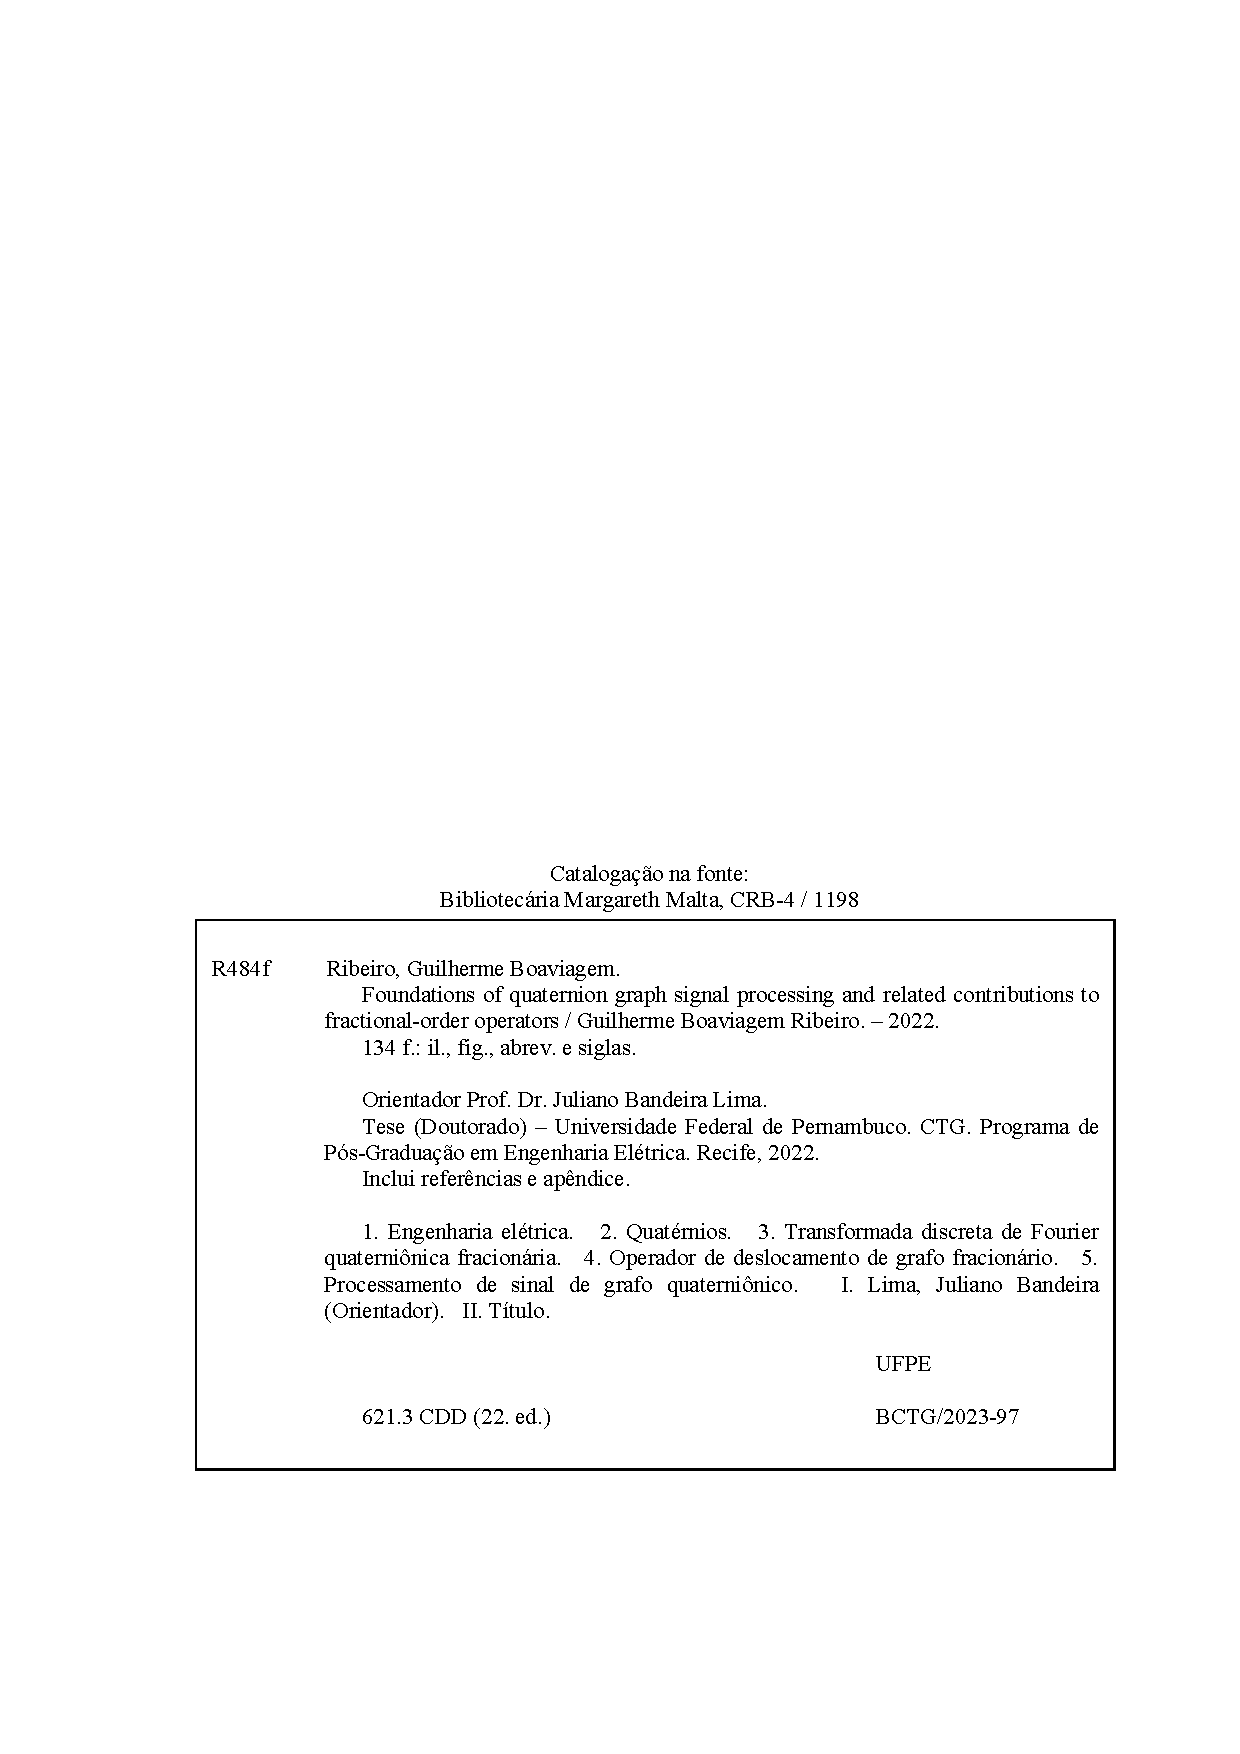
\includepdf[pages={1}]{./frontmatter/ficha_catalografica.pdf}
% \end{fichacatalografica}


% ---
% Inserir errata
% ---
%\begin{errata}
%Elemento opcional da \citeonline[4.2.1.2]{NBR14724:2011}. Exemplo:
%
%\vspace{\onelineskip}
%
%FERRIGNO, C. R. A. \textbf{Tratamento de neoplasias ósseas apendiculares com
%reimplantação de enxerto ósseo autólogo autoclavado associado ao plasma
%rico em plaquetas}: estudo crítico na cirurgia de preservação de membro em
%cães. 2011. 128 f. Tese (Livre-Docência) - Faculdade de Medicina Veterinária e
%Zootecnia, Universidade de São Paulo, São Paulo, 2011.
%
%\begin{table}[htb]
%\center
%\footnotesize
%\begin{tabular}{|p{1.4cm}|p{1cm}|p{3cm}|p{3cm}|}
%  \hline
%   \textbf{Folha} & \textbf{Linha}  & \textbf{Onde se lê}  & \textbf{Leia-se}  \\
%    \hline
%    1 & 10 & auto-conclavo & autoconclavo\\
%   \hline
%\end{tabular}
%\end{table}
%
%\end{errata}
% ---

% ---
% Inserir folha de aprovação
% ---

\begin{folhadeaprovacao}
    \begin{center}
% {\ABNTEXchapterfont\large\imprimirautor}
\MakeUppercase{\rmfamily\mdseries\normalsize\imprimirautor}

\vspace*{\fill}\vspace*{\fill}
\begin{center}
    % \ABNTEXchapterfont\bfseries\Large\imprimirtitulo
    \MakeUppercase{\rmfamily\bfseries\normalsize\imprimirtitulo}
\end{center}
\vspace*{\fill}

\hspace{.45\textwidth}
\begin{minipage}{.5\textwidth}
    \imprimirpreambulo
\end{minipage}%
\vspace*{\fill}
\end{center}

Este trabalho foi aprovado em 23/12/2022 pela seguinte banca de doutorado:

\assinatura{\textbf{\imprimirorientador} \\ (Orientador and Examinador Interno) \\ Universidade Federal de Pernambuco}
\assinatura{\textbf{Prof. Dr. Alfred Doe} \\ (Examinador Interno) \\ Universidade Federal de Pernambuco}
\assinatura{\textbf{Prof. Dr. Bernard Doe} \\ (Examinador Interno) \\ Universidade Federal de Pernambuco}
\assinatura{\textbf{Prof. Dr. Charles Doe} \\ (Examinador Externo) \\ University of Luxembourg}
\assinatura{\textbf{Prof. Dr. Earl Doe} \\ (Examinador Externo) \\ Federal University of Esp\'irito Santo}

\end{folhadeaprovacao}
% ---

\begin{dedicatoria}
    \vspace*{\fill}
\centering
\noindent
Dedicatória.
\vspace*{\fill}
\end{dedicatoria}

\begin{agradecimentos}
    % !TEX root = ../thesis-example.tex
%
% \pdfbookmark[0]{Agradecimentos}{Agradecimentos}
% \chapter*{Agradecimentos}
% \label{sec:acknowledgement}
%\vspace*{-10mm}

\begin{openingquote}
    Insisto: na simplicidade do teu trabalho habitual, nos detalhes monótonos de cada dia, tens que descobrir o segredo - para tantos escondido - da grandeza e da novidade: o Amor. \cite[n. 489]{escriva2016sulco}
\end{openingquote}

\lipsum[1-3]
\end{agradecimentos}

\begin{epigrafe}
    \vspace*{\fill}
\begin{openingquote}
Algebra is generous, she often gives more than is asked of her.
\cite{bulletinams}    
\end{openingquote}
\end{epigrafe}
% ---

%
%% resumo em inglês
\begin{resumo}[Abstract]
    \begin{otherlanguage*}{english}
    
% !TEX root = ../thesis-example.tex
%
% \pdfbookmark[0]{Abstract}{Abstract}
% \chapter*{Abstract}
% \label{sec:abstract}
%\vspace*{-10mm}

\lipsum[2]
\vspace{1em}

Keywords: quaternions; fractional quaternion discrete Fourier transform; fractional graph shift operator; quaternion graph signal processing.

    \end{otherlanguage*}
\end{resumo}

\begin{resumo}[Resumo]
    \begin{otherlanguage*}{portuguese}
    
% !TEX root = ../thesis-example.tex
%
% \pdfbookmark[0]{Abstract}{Abstract}
% \chapter*{Abstract}
% \label{sec:abstract}
%\vspace*{-10mm}

\lipsum[5]
\vspace{1em}

Palavras-chave: quatérnios; transformada discreta de Fourier quaterniônica fracionária; operador de deslocamento de grafo fracionário; processamento de sinal de grafo quaterniônico.
    \end{otherlanguage*}
\end{resumo}

% resumo em francês 
%\begin{resumo}[Résumé]
%\begin{otherlanguage*}{french}
%Il s'agit d'un résumé en français.
%
%\textbf{Mots-clés}: latex. abntex. publication de textes.
%\end{otherlanguage*}
%\end{resumo}

% resumo em espanhol
%\begin{resumo}[Resumen]
%\begin{otherlanguage*}{spanish}
%Este es el resumen en español.
%
%\textbf{Palabras clave}: latex. abntex. publicación de textos.
%\end{otherlanguage*}
%\end{resumo}
% ---

% ---
% inserir lista de ilustrações
% ---
\pdfbookmark[0]{\listfigurename}{lof}
\listoffigures*
\cleardoublepage
% ---

% ---
% inserir lista de quadros
% ---
%\pdfbookmark[0]{\listofquadrosname}{loq}
%\listofquadros*
%\cleardoublepage
% ---

% ---
% inserir lista de tabelas
% ---
%\pdfbookmark[0]{\listtablename}{lot}
%\listoftables*
%\cleardoublepage
% ---

% ---
% inserir lista de abreviaturas e siglas
% ---
\begin{siglas}
    % \pdfbookmark[0]{Abbreviations}{Abbreviations}
% \chapter*{List of abbreviations}
% \label{sec:acronimos}
% %\vspace*{-10mm}

% \begin {description}[leftmargin=8em,style=nextline]
\item[DFT] Discrete Fourier Transform.
\item[DSP] Digital Signal Processing.
\item[FIR] Finite Impulse Response.

\end{siglas}
% ---

% ---
% inserir lista de símbolos
% ---
\begin{simbolos}
    % \pdfbookmark[0]{List of symbols}{symbols}
% \chapter*{List of symbols}
% \label{sec:symbols}
% %\vspace*{-10mm}


\item[$ \mathbf{A} $] Matriz de adjacência ponderada do grafo.
\item[$ \mathbf{L} $] Matriz Laplaciana do grafo.
\item[$ \mathbf{\Lambda}, \mathbf{J} $] Respectivamente a matriz de autovalores (se existir) e a matriz de Jordan da matriz de adjacência do grafo.
\item[$ \mathbf{V} $] A matriz de autovetores (possivelmente generalizada) da matriz de adjacência do grafo.
\item[$\mathcal{R}e \{ x \}$] Parte real do número complexo $x$.
\item[$\mathcal{I}m \{ x \}$] Parte imaginária do número complexo $x$.
\item[$ \overline{x} $] Conjugado do número complexo (ou quaterniônico) $x$. Se vetores ou matrizes forem usados em vez de $x$, a conjugação é realizada em cada uma de suas entradas.
\item[$\mathbf{M}^T$] Transposta da matriz $\mathbf{M}$.
\item[$\mathbf{M}^H$] Transposta conjugada da matriz $\mathbf{M}$.
\item[$\mathbb{R}$, $\mathbb{C}$ e $\mathbb{H}$] Respectivamente, o conjunto dos números reais, complexos e (hamiltonianos) quaterniônicos. Por associação, também podemos nos referir ao respectivo \emph{skew field}.
\end{simbolos}


% ---

% ---
% inserir o sumario
% ---
\pdfbookmark[0]{\contentsname}{toc}
\tableofcontents*
\cleardoublepage
% ---



% ----------------------------------------------------------
% ELEMENTOS TEXTUAIS
% ----------------------------------------------------------
\textual

\chapter{Introduction}
\label{ch:Intro}

Signal processing often interweaves pure mathematics and engineering. One of its concerns is the \textit{representation} of signals (functions) and how different representations may be explored to better manipulate such signals. The spectral analysis via Fourier and similar transforms, for instance, aims to project the signal onto a domain in which the energy support is more compact (compression), or in which some frequencies are easier to be removed (filtering), or yet in which some relevant features may be created (feature engineering for machine learning problems), among others \cite{oppenheim1999discrete, rabiner2010theory, graf2015features, vergin1999generalized}.

\lipsum[1-2]
\chapter{A review on quaternion algebra and its Fourier transform}
\label{ch:reviewQuat}

In 1833, at the age of 28, Willian Rowan Hamilton presented to the Royal Irish Academy (RIA) a work in which complex numbers were treated as ordered pairs of real numbers, given the appropriate definition of operations.\footnote{The results were published in 1837, in the paper \emph{Theory of Conjugate Functions, or Algebraic Couples; with a Preliminary and Elementary Essay on Algebra as the Science of Pure Time} \cite{hamilton1837theory}.} In the following years, he struggled to extend the complex field into a normed division algebra over triples, but soon realized that, as much as his attempts were inventive, the resulting algebra\footnote{An \textit{algebra over a field}, or simply \textit{algebra}, is a vector space over a field with a bilinear multiplication (that is, the multiplication distributes over the addition and the associativity is valid for multiplication) \cite{schafer1955introduction}.} was not closed under multiplication. We can see this through a simple example \cite{santos2011algebra}: let it be the set $\mathbb{F} = \{ a + b \qi + c \qj  \ | \ (a, b, c) \in \mathbb{R}^3\}$, with $\qi^2 = \qj^2 = -1$ and $\qi \neq \qj$. Since $\qi, \qj \in \mathbb{F}$, so there should exist $x, y, z \in \mathbb{R}$ so that
\begin{equation}
    \qi \qj = x + y \qi + z \qj.
    \label{eq:demonstration01}
\end{equation}

Multiplying by $\qi$ both sides of the equation,
\begin{equation}
    \qi^2 \qj = \qi x + \qi^2 y + z (\qi \qj),
\end{equation}
and using (\ref{eq:demonstration01}) it yields,
\begin{equation}
    - \qj = \qi x - y + z (x + y \qi + z \qj)
    \iff
    (zx - y) + \qi (x + zy) + \qj (z^2 + 1) = 0.
\end{equation}
That is: $z \notin \mathbb{R}$ and $ \qi \qj \notin \mathbb{F} $, proving that such algebraic structure is not closed under multiplication.

Only a decade later, in 1843, while walking by the roads in Dublin toward the RIA, ``an electric circuit seemed to close, and a spark flashed forth,'' as he would say. He had conceived the four-dimensional structure required to the desired algebra, creating the quaternions. Moved by excitement, he craved on the stone below Broome Bridge, in Cabra (Dublin), the equations that define the relations between the canonical basis elements of quaternions.\footnote{Close to the original site of the inscriptions, the RIA placed a commemorative plaque in 1958, with the same writings.} This creation, made possible by an insight in 1843, is found accross most of this work. The following sections lead the reader through the foundations of quaternion algebra and quaternion signal analysis.


\section{Introduction to the quaternion algebra}

Quaternions are numbers $q \in \mathbb{H}$ in the form
\begin{equation}
    q = a + b\qi + c\qj + d\qk,
    \label{eq:q}
\end{equation}
in which $a, b, c, d \in \mathbb{R}$, holding true the fundamental relations:
\begin{equation}
    \label{eq:fund_rel}
    \begin{aligned}
        \qi ^2 = \qj^2 & =\qk^2 = \qi \qj \qk = -1.
    \end{aligned}
\end{equation}

The multiplication rules between  $ \qi $, $ \qj $ and $ \qk $ follow directly from (\ref{eq:fund_rel}), resembling those between orthonormal basis vectors from $ \mathbb{R}^3 $ and the vector product: the product between two of them yields the third, the sign being determined from the operands order. For instance, to find the result of $ \qi \qj $ one may start from (\ref{eq:fund_rel}) and write
\begin{equation}
    \begin{aligned}
        \qi \qj \qk                         & = -1   \\
        \qi \qj \underbrace{\qk \qk}_{= -1} & = -\qk \\
        \qi \qj                             & = \qk.
    \end{aligned}
\end{equation}
Similarly, to find $ \qj \qi $,
\begin{equation}
    \begin{aligned}
        \qi \qj \qk     & = -1        \\
        \qi \qi \qj \qk & = -\qi      \\
        - \qj \qk       & = - \qi     \\
        \qj \qj \qk     & =  \qj \qi  \\
        - \qk           & =  \qj \qi. \\
    \end{aligned}
\end{equation}
Fig. \ref{fig:quatmult} depicts the order in which the product between any pair in the triplet $ \qi $, $ \qj $ and $ \qk $ yields the third one, with positive sign. All three units commute with real numbers. The most relevant consequence, therefore, of (\ref{eq:fund_rel}), is that the quaternion product is \textit{noncommutative}. In fact, it is the first example of noncommutative normed division algebra in history \cite{kleiner2007history}.

\begin{figure}
    \centering
    \caption{Illustration of the multiplication rule between the imaginary units $ \qi $, $ \qj $ and $ \qk $.}
    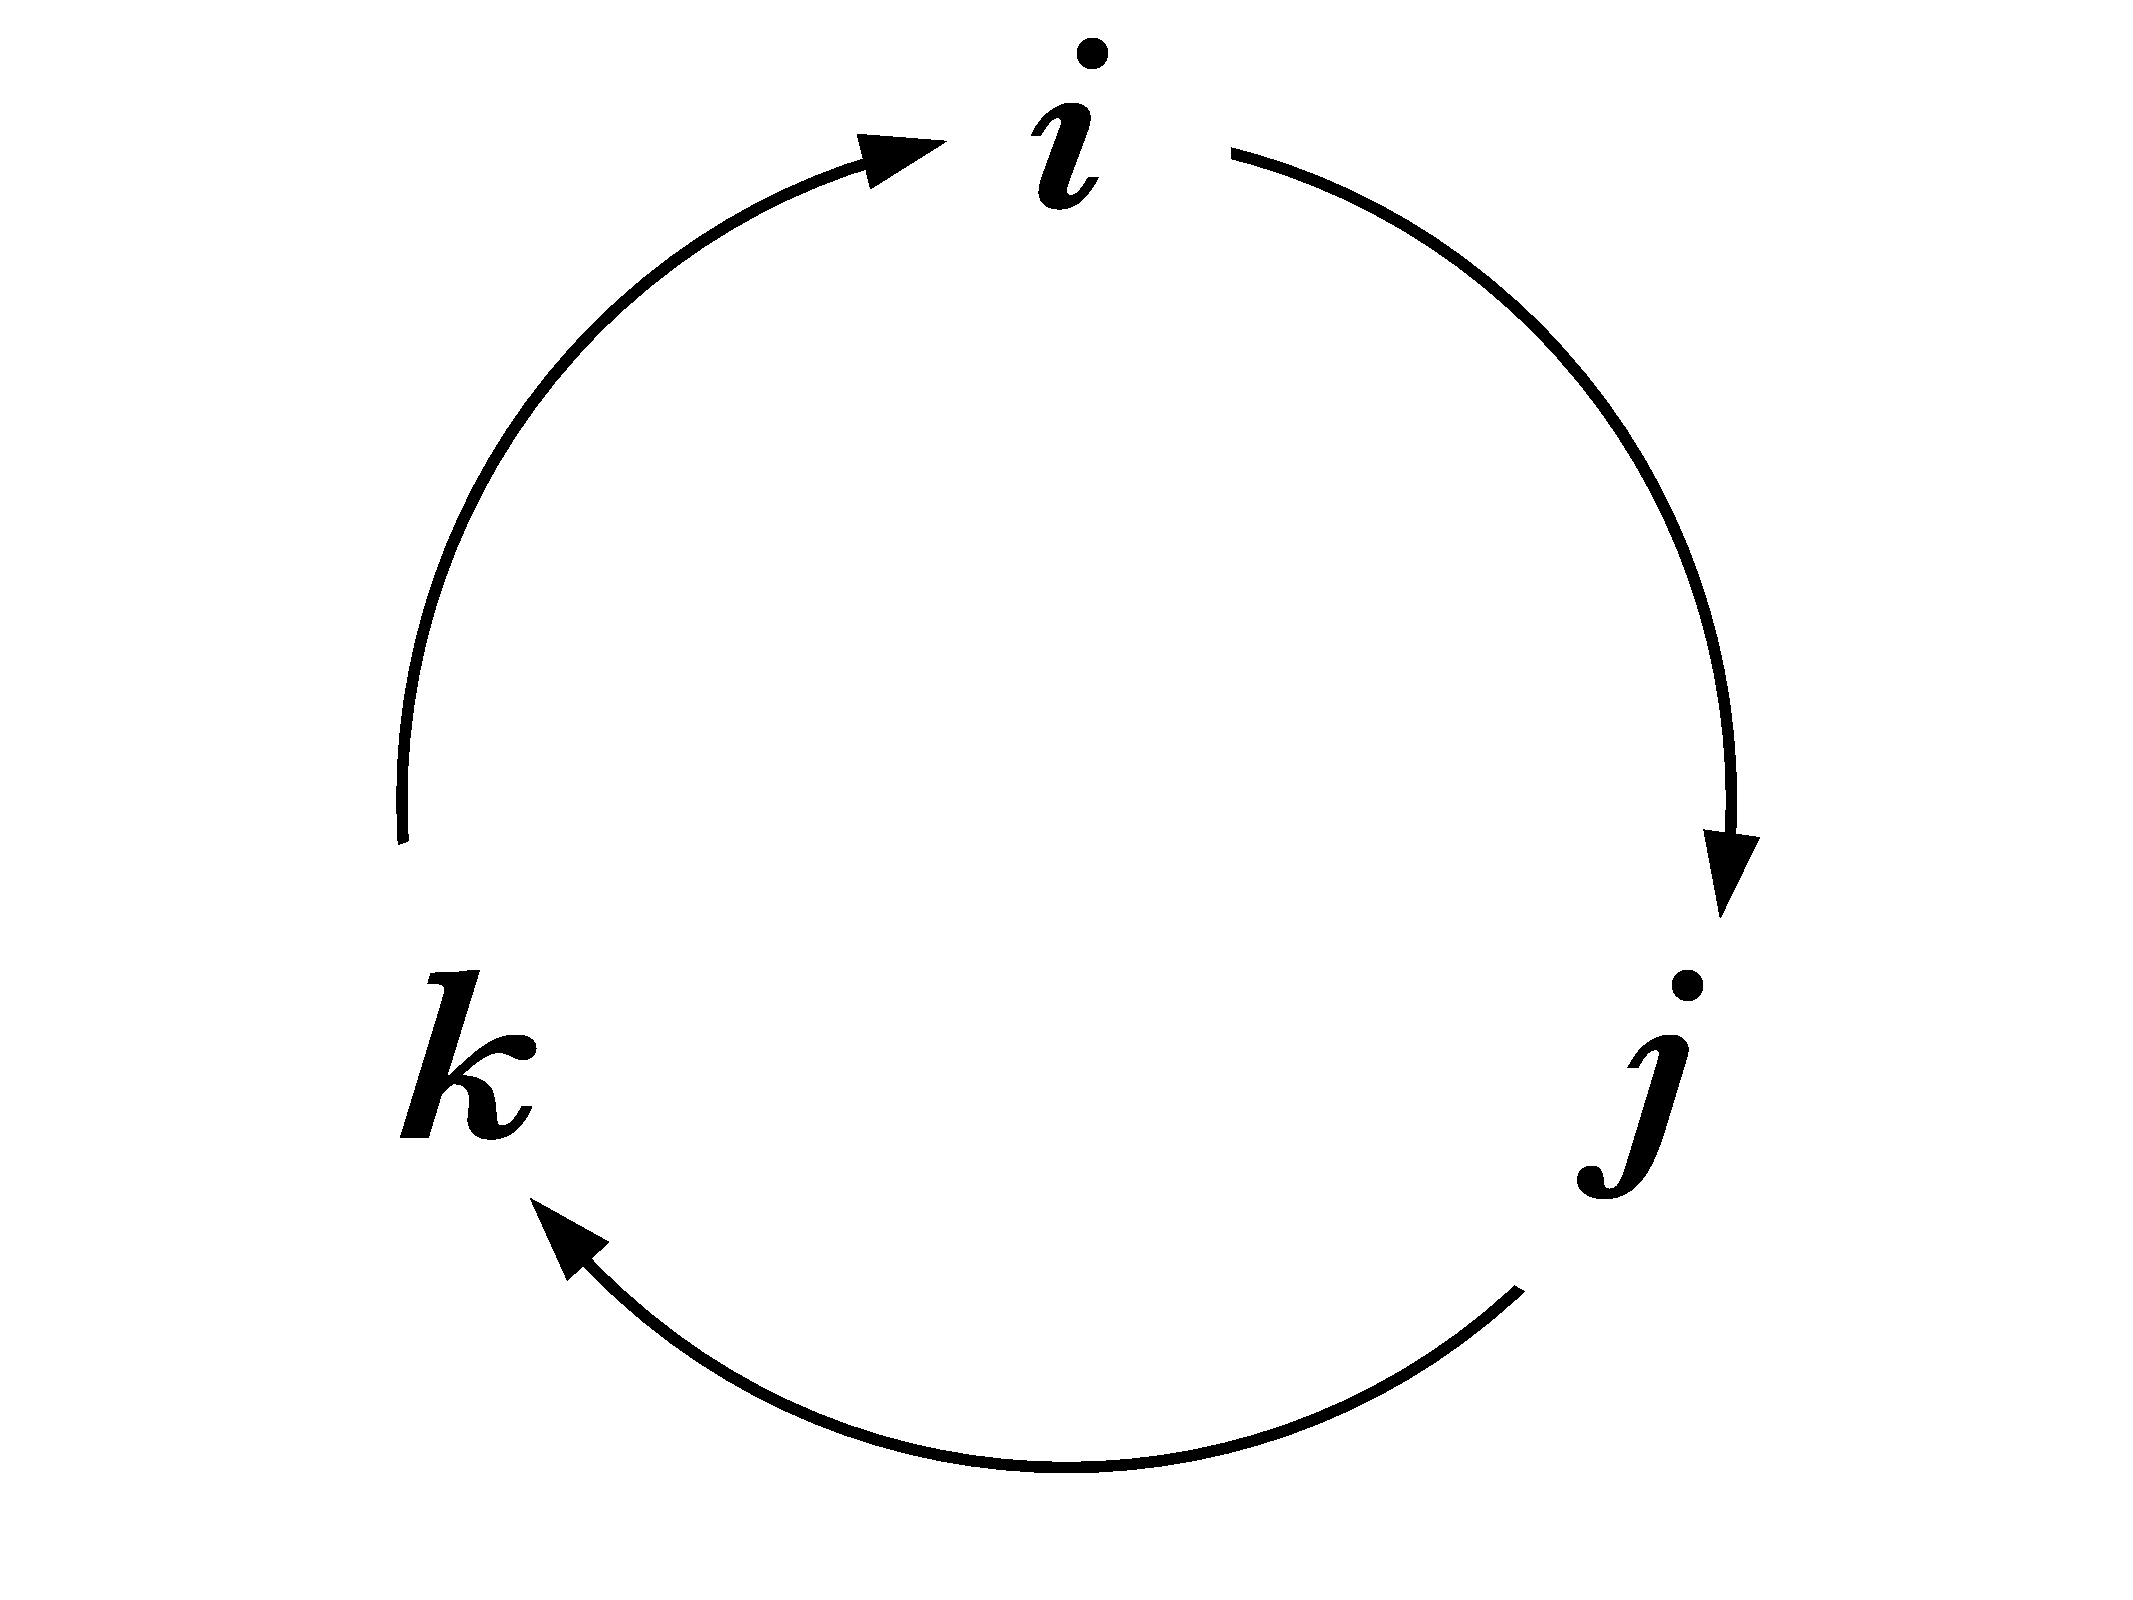
\includegraphics[width=0.2\linewidth]{Figures/quaternion_multiplication.pdf}
    \floatsource
    \label{fig:quatmult}
\end{figure}
\chapter{Conclusion}
\label{ch:conclusion}

\begin{openingquote}
    Quaternions came from Hamilton after his really good work had been done; and, though beautifully ingenious, have been an unmixed evil to those who have touched them in any way [...].
    \cite[quoting directly Lord Kelvin, in letter to Hatward, 1892]{altmann1989hamilton}
\end{openingquote}

\lipsum[1-2]

% ----------------------------------------------------------
% Finaliza a parte no bookmark do PDF
% para que se inicie o bookmark na raiz
% e adiciona espaço de parte no Sumário
% ----------------------------------------------------------
\phantompart

% ---
% Conclusão
% ---
%\chapter{Conclusão}
% ---

%\lipsum[31-33]
%Conclus\~ao.

% ----------------------------------------------------------
% ELEMENTOS PÓS-TEXTUAIS
% ----------------------------------------------------------
\postextual
% ----------------------------------------------------------

% ----------------------------------------------------------
% Referências bibliográficas
% ----------------------------------------------------------
%\bibliographystyle{ieeetr}
\bibliography{mybib}
%\addcontentsline{toc}{section}{Refer\^encias}

% ----------------------------------------------------------
% Glossário
% ----------------------------------------------------------
%
% Consulte o manual da classe abntex2 para orientações sobre o glossário.
%
%\glossary

% ----------------------------------------------------------
% Apêndices
% ----------------------------------------------------------

% ---
% Inicia os apêndices
% ---
\begin{apendicesenv}

    % Imprime uma página indicando o início dos apêndices
    % \partapendices

    % ----------------------------------------------------------
    \chapter{Mapeando equações de $ \mathbb{H} $ para $ \mathbb{C} $}
\label{ch:AppendixA}
% ----------------------------------------------------------

\lipsum[1-2]

\end{apendicesenv}
% ---


% ----------------------------------------------------------
% Anexos
% ----------------------------------------------------------

% ---
% Inicia os anexos
% ---
%\begin{anexosenv}
%
%% Imprime uma página indicando o início dos anexos
%\partanexos
%
%% ---
%\chapter{Morbi ultrices rutrum lorem.}
%% ---
%\lipsum[30]
%
%% ---
%\chapter{Cras non urna sed feugiat cum sociis natoque penatibus et magnis dis
%parturient montes nascetur ridiculus mus}
%% ---
%
%\lipsum[31]
%
%% ---
%\chapter{Fusce facilisis lacinia dui}
%% ---
%
%\lipsum[32]
%
%\end{anexosenv}

%---------------------------------------------------------------------
% INDICE REMISSIVO
%---------------------------------------------------------------------
\phantompart
\printindex
%---------------------------------------------------------------------

\end{document}
